\documentclass[11pt]{article}

\usepackage[margin=1in]{geometry}
\usepackage{amsmath}
\usepackage{graphicx}
\usepackage{booktabs}
\usepackage{hyperref}
\usepackage{authblk}
\usepackage[T1]{fontenc}

\title{Order Flow Imbalance and Short-Horizon BTC/USDT Returns:\\ A Signal That Kept Needing More Scrutiny}
\author[Your Name]{Your Name}
\date{Draft --- 2026-07-22}

\begin{document}
\maketitle

\begin{abstract}
We test whether order-flow imbalance (OFI), defined per Cont, Kukanov \& Stoikov (2014), predicts short-horizon (1--10 second) mid-price returns in BTC/USDT, using L2 order-book data reconstructed from Binance.US's diff-depth stream. Across three successive extensions of the same capture, evaluated with an identical pipeline, the result changed twice. An initial $\sim$7-day sample (588{,}417 windows) showed statistically significant positive out-of-sample $R^2$ (0.17\%--1.00\%), decaying monotonically with horizon and surviving a permutation placebo check. Extending to $\sim$9 days (785{,}966 windows) reversed this: pooled $R^2$ turned negative or indistinguishable from zero at every horizon. Extending further to $\sim$16 days, while also fixing two data-pipeline issues found via the same fold-level diagnostics used throughout (a silent gap-detection defect, \S2.2; and unmasked targets computed across a multi-day collector outage, \S4.4) and adding purge/embargo to the walk-forward splitter, reversed it again: pooled out-of-sample $R^2$ is positive at every horizon for both feature variants (0.13\%--0.93\%), with confidence intervals excluding zero except for best-level OFI at 5s, and the result again survives a placebo check. Fold-level decomposition throughout shows a coefficient that never changes sign and drifts smoothly, while fold-level fit quality is noisy and only net-favorable with enough pooled data. We read this as a small, real, direction-consistent effect that is difficult to detect reliably out-of-sample below roughly two weeks of single-symbol, single-venue data --- and as a demonstration that in this regime, a single walk-forward result, however clean, should be treated as provisional until it has survived at least one deliberate attempt to break it.
\end{abstract}

\section{Introduction}

Cont, Kukanov \& Stoikov (2014) show that order-flow imbalance --- the net directional pressure implied by changes at the best bid and ask --- has explanatory power for contemporaneous price changes in equities. A natural follow-up question, and the one this project tests, is whether OFI has \emph{predictive} power for near-future returns at the sub-10-second horizons relevant to a market maker or short-horizon signal researcher, in a different asset class and venue: BTC/USDT spot on Binance.US.

\paragraph{Hypothesis.} OFI has statistically significant predictive power for BTC/USDT mid-price returns at sub-10-second horizons, out-of-sample, with $R^2$ decaying monotonically as the horizon increases.

We test this with walk-forward validation exclusively --- no shuffled cross-validation --- Newey-West HAC standard errors for the autocorrelation inherent in overlapping-window returns, purge/embargo to remove label overlap at fold boundaries, and moving-block bootstrap confidence intervals for the out-of-sample $R^2$ itself. Full source is in the accompanying repository; every reconstruction and evaluation step is unit tested against synthetic data with known-correct answers.

\section{Data}

\subsection{Collection}

We collect BTC/USDT L2 order-book data from Binance.US: the \texttt{<symbol>@depth} diff-update WebSocket stream (event-driven, sub-second granularity), \texttt{<symbol>@trade} for executed trades, and periodic (15-minute) REST \texttt{GET /api/v3/depth} snapshots used to (re)synchronize the local book.

The collector is a foreground process with automatic WebSocket reconnect-on-disconnect, but it is not a background service --- closing its terminal kills it. This happened once during collection: the collector ran continuously from 2026-07-06 00:05:49 UTC, stopped cleanly (no error, no crash traceback) at 2026-07-16 03:55 UTC, and was restarted at 2026-07-20 00:0x UTC, leaving a gap of roughly 3 days 21 hours in the raw capture. \S4.4 describes how this gap was found --- not from an operational check, but from a walk-forward fold behaving impossibly --- and how the analysis pipeline now handles it. The full capture used in \S4.3 onward runs through 2026-07-22 03:24:08 UTC (3{,}788{,}566 reconstructed book states); \S4.1 and \S4.2 use earlier, shorter cutoffs of the same ongoing capture, predating the outage, exactly as originally analyzed.

\subsection{Book reconstruction and a data-quality finding}

The local order book is reconstructed offline from the raw capture by replaying diff events against periodic snapshots, following Binance's documented buffer/snapshot/resync procedure. This produced a directly relevant finding worth reporting as part of the data-quality record: Binance publishes an optional \texttt{pu} (previous-update-id) field on the diff stream specifically to let a client detect a dropped or reordered message and resync. On Binance.US, \texttt{pu} is absent from every single event (confirmed across a random sample of 7{,}515 events across 15 capture files) --- a venue-specific behavior not documented anywhere we found, and different from Binance.com's stream. Because the original reconstruction code only checked sequence continuity when \texttt{pu} was present, gap detection was silently disabled for the entire capture: dropped messages around WebSocket reconnects went undetected instead of triggering a resync, leaving stale price levels on one side of the book while the other kept moving. This produced a crossed (bid $\geq$ ask) spread on 218{,}006 of 1{,}955{,}157 reconstructed book states (11.2\%), concentrated in bursts around reconnect events rather than spread uniformly.

The fix falls back to Binance's classic pre-\texttt{pu} algorithm when \texttt{pu} is absent: the next event's first update ID (\texttt{U}) must equal the previous event's final update ID (\texttt{u}) plus one. After the fix, the same capture reconstructs with \textbf{zero} crossed-spread violations across 1{,}948{,}728 book states, and correctly detects real sequence gaps that had previously gone unnoticed (0 gaps detected before the fix; 468 real gaps detected after, on the same underlying data). We flag this explicitly because it is exactly the kind of silent, non-crashing correctness bug that would otherwise inject noise into every downstream OFI number without any obvious symptom --- the pipeline never raised an exception; only an explicit invariant check (spread must be positive) caught it.

\section{Methodology}

\subsection{OFI definition}

At the best bid/ask (level 1), OFI follows Cont, Kukanov \& Stoikov (2014) directly. For consecutive book states, with bid/ask price and size $(P^B, q^B)$ / $(P^A, q^A)$:

\begin{equation}
\Delta W^B_n =
\begin{cases}
q^B_n & P^B_n > P^B_{n-1} \\
q^B_n - q^B_{n-1} & P^B_n = P^B_{n-1} \\
-q^B_{n-1} & P^B_n < P^B_{n-1}
\end{cases}
\qquad
\Delta W^A_n =
\begin{cases}
-q^A_{n-1} & P^A_n > P^A_{n-1} \\
q^A_n - q^A_{n-1} & P^A_n = P^A_{n-1} \\
q^A_n & P^A_n < P^A_{n-1}
\end{cases}
\end{equation}

\begin{equation}
\text{OFI}_n = \Delta W^B_n - \Delta W^A_n
\end{equation}

We additionally construct a \textbf{depth-weighted 5-level variant}, extending the level-1 formula to each of the top 5 book levels (matched by depth rank, not price identity) and combining them with weight $1/i$ for level $i$: the touch dominates, but deeper levels still contribute, down-weighted rather than dropped. This weighting is a design choice made for this study, not a literature-standard constant --- the original paper defines only the level-1 statistic.

A reconstruction row immediately following a resync (see \S2.2) has no well-defined predecessor state, so its OFI is undefined (excluded, not zero) rather than computed against stale pre-gap data.

\subsection{Windows, horizons, and the no-lookahead contract}

Event-level OFI is summed into fixed, non-overlapping 1-second tumbling windows. For each window $t$, we compute forward log-returns at horizons $h \in \{1, 2, 5, 10\}$ seconds:

\begin{equation}
r_{t,h} = \log(\text{mid}_{t+h}) - \log(\text{mid}_t)
\end{equation}

A window's OFI feature uses only events up to and including that window's own end; its target uses mid-price at that window and a strictly later one. Nothing between $t$ and $t+h$ that wasn't already summarized into an earlier window's OFI leaks into the feature. This is verified directly in unit tests (\texttt{tests/test\_features.py}), including that the trailing $h$ windows of each horizon column are \texttt{NaN} rather than filled or wrapped.

A window with zero captured events (a short quiet moment, or, as in \S4.4, an extended collection outage) has its mid-price forward-filled from the last real observation and is flagged \texttt{mid\_price\_filled}. A target is forced to \texttt{NaN} whenever \emph{either} its origin or destination window carries that flag --- a ``return'' computed off a stale filled price is not a real observation of market behavior, and, as \S4.4 shows, silently keeping such targets is not harmless padding: a long enough gap manufactures thousands of fabricated exactly-zero returns paired with exactly-zero OFI, which is fabricated data that can dominate a single fold's statistics.

\subsection{Walk-forward validation, with purge and embargo}

We use purely chronological, expanding-window walk-forward validation: the first 50\% of the sample is a minimum training burn-in, and the remaining 50\% is split into 5 contiguous, non-overlapping test folds. Fold $k$'s training set is every observation strictly before that fold; fold $k+1$'s training set is a superset of fold $k$'s (it expands to include fold $k$ itself). No shuffled cross-validation is used anywhere in this study.

Starting with the \S4.3 extension, we additionally trim the trailing edge of each fold's training set following L\'opez de Prado (\emph{Advances in Financial Machine Learning}, ch.\ 7): \textbf{purge} drops exactly the trailing training rows whose $h$-bin-ahead label reaches into the test period (a row at $\text{test\_start}-1$ with a 10-bin-ahead target technically has a label computed from inside the test window); \textbf{embargo} drops a further, equal-sized buffer beyond the purge as defense-in-depth against residual short-range serial correlation that label-purging alone doesn't address. In this pure forward-chaining design, training data is always strictly earlier than test data for any given fold's own fit, so only the pre-test boundary needs trimming --- there is no post-test training data within a single fold for a symmetric embargo to protect against. \S4.1--4.2 predate this addition; its effect, measured directly on the \S4.3 sample, was small (pooled $R^2$ moved by roughly 0.01--0.05 percentage points versus an unpurged rerun on the same data).

The model is plain OLS: $r_{t,h} = \alpha + \beta \cdot \text{OFI}_t + \varepsilon_t$, fit independently on each fold's training data.

\subsection{Statistical inference}

\textbf{Out-of-sample $R^2$.} We report the Campbell \& Thompson (2008) out-of-sample $R^2$, benchmarked against the \emph{training-period mean} forecast (not zero): $R^2_{oos} = 1 - \text{SSE}_{model} / \text{SSE}_{benchmark}$, pooled across all 5 test folds. Predicting zero would silently assume the true unconditional mean return is exactly zero, which is not given and would inflate $R^2$ by whatever the true drift is.

\textbf{Newey-West HAC significance.} Because both OFI and short-horizon returns are autocorrelated (order flow clusters; horizons longer than the sampling window make consecutive targets overlap), we fit OLS on the full sample with a Newey-West heteroskedasticity-and-autocorrelation-consistent covariance matrix (\texttt{maxlags} set to at least twice the horizon-to-window ratio) rather than relying on ordinary standard errors, which would understate the true uncertainty and overstate significance.

\textbf{Block bootstrap.} We construct a 95\% confidence interval for the pooled out-of-sample $R^2$ via moving block bootstrap (Kunsch, 1989): contiguous blocks of consecutive (actual, predicted, benchmark) triples are resampled with replacement (block size scaled to the horizon), preserving local serial dependence that an i.i.d.\ bootstrap would average away.

We treat in-sample significance and out-of-sample $R^2$ as answering different questions and report both rather than conflating them: a coefficient can be significant in-sample yet fail to generalize out-of-sample, which is precisely what \S4 documents.

\section{Results}

\subsection{Initial analysis ($\sim$7 days, 588{,}417 windows)}

Using book states reconstructed through 2026-07-12 19:32 UTC:

\begin{table}[h]
\centering
\begin{tabular}{llrrr}
\toprule
Feature & Horizon & OOS $R^2$ & 95\% Bootstrap CI & NW $t$-stat \\
\midrule
Best-level OFI & 1s & +0.58\% & [+0.37\%, +0.81\%] & +30.1 \\
Best-level OFI & 2s & +0.47\% & [+0.32\%, +0.65\%] & +28.1 \\
Best-level OFI & 5s & +0.30\% & [+0.16\%, +0.45\%] & +23.1 \\
Best-level OFI & 10s & +0.17\% & [+0.07\%, +0.28\%] & +16.3 \\
Depth-weighted 5-level OFI & 1s & +1.00\% & [+0.76\%, +1.26\%] & +37.4 \\
Depth-weighted 5-level OFI & 2s & +0.86\% & [+0.68\%, +1.04\%] & +35.1 \\
Depth-weighted 5-level OFI & 5s & +0.60\% & [+0.41\%, +0.76\%] & +27.1 \\
Depth-weighted 5-level OFI & 10s & +0.37\% & [+0.23\%, +0.54\%] & +19.9 \\
\bottomrule
\end{tabular}
\caption{Initial $\sim$7-day out-of-sample results.}
\end{table}

This matched the stated hypothesis exactly: positive, significant, monotonically-decaying-with-horizon out-of-sample $R^2$, with the multi-level variant consistently outperforming best-level alone. As an additional robustness check, we permuted the OFI feature (breaking its temporal alignment with the target while preserving its marginal distribution) and reran the identical pipeline: $R^2$ collapsed from +0.58\%/+0.30\% (1s/5s, best-level) to $-$0.0017\%/$-$0.0001\%, confirming the result was not a mechanical artifact of the window/target construction. No purge/embargo yet (\S3.3).

\subsection{Extended analysis ($\sim$9 days, 785{,}966 windows)}

Two additional days of capture (through 2026-07-15 02:25 UTC, still predating the collector outage in \S2.1) were added and the identical pipeline rerun with no code changes:

\begin{table}[h]
\centering
\begin{tabular}{llrrr}
\toprule
Feature & Horizon & OOS $R^2$ & 95\% Bootstrap CI & NW $t$-stat \\
\midrule
Best-level OFI & 1s & $-$0.18\% & [$-$0.42\%, +0.07\%] & +27.7 \\
Best-level OFI & 2s & $-$0.22\% & [$-$0.45\%, +0.01\%] & +27.2 \\
Best-level OFI & 5s & $-$0.30\% & [$-$0.47\%, $-$0.12\%] & +24.0 \\
Best-level OFI & 10s & $-$0.18\% & [$-$0.34\%, $-$0.02\%] & +18.7 \\
Depth-weighted 5-level OFI & 1s & +0.10\% & [$-$0.19\%, +0.43\%] & +36.6 \\
Depth-weighted 5-level OFI & 2s & $-$0.01\% & [$-$0.29\%, +0.29\%] & +36.1 \\
Depth-weighted 5-level OFI & 5s & $-$0.17\% & [$-$0.38\%, +0.05\%] & +30.9 \\
Depth-weighted 5-level OFI & 10s & $-$0.14\% & [$-$0.36\%, +0.08\%] & +23.9 \\
\bottomrule
\end{tabular}
\caption{Extended $\sim$9-day out-of-sample results.}
\end{table}

Every configuration is now negative or statistically indistinguishable from zero out-of-sample. Best-level OFI is negative at every horizon, with the CI excluding zero (on the negative side) at 5s and 10s. Newey-West $t$-statistics remain enormous throughout --- full sample size makes in-sample significance easy to achieve and, on its own, uninformative about predictive usefulness, which is precisely the gap between \S3.4's two questions.

A first fold-level decomposition at this stage (best-level OFI, 1s horizon) showed a coefficient that never changed sign across folds (0.000049 $\to$ 0.000037, monotonically shrinking) while fold-level out-of-sample fit alternated sign with no visible trend (+0.66\%, $-$0.54\%, $-$0.13\%, +0.29\%, $-$0.95\%) --- swings large relative to the point estimates themselves, suggestive of a real-but-small effect rather than a reversing one, but not yet distinguishable from ``no effect'' on this sample.

\subsection{Second extension ($\sim$16 days, purge/embargo, gap-aware targets)}

Collection continued (through a mid-collection outage, \S2.1) to roughly 16 days (3{,}788{,}566 reconstructed book states, 2026-07-06 00:05:49 UTC through 2026-07-22 03:24:08 UTC; 1{,}394{,}300 one-second windows before gap masking). Before rerunning, we made two changes, both described in full in \S3.3 and \S4.4: added purge/embargo to the walk-forward splitter, and fixed the target computation to exclude any window touching the collector-outage gap rather than silently treating a forward-filled flat price as a real observation.

\begin{table}[h]
\centering
\begin{tabular}{llrrr}
\toprule
Feature & Horizon & OOS $R^2$ & 95\% Bootstrap CI & NW $t$-stat \\
\midrule
Best-level OFI & 1s & +0.30\% & [+0.06\%, +0.52\%] & +32.3 \\
Best-level OFI & 2s & +0.24\% & [+0.05\%, +0.42\%] & +32.1 \\
Best-level OFI & 5s & +0.13\% & [$-$0.06\%, +0.27\%] & +28.3 \\
Best-level OFI & 10s & +0.14\% & [+0.03\%, +0.26\%] & +22.3 \\
Depth-weighted 5-level OFI & 1s & +0.93\% & [+0.67\%, +1.19\%] & +44.0 \\
Depth-weighted 5-level OFI & 2s & +0.82\% & [+0.58\%, +1.04\%] & +43.6 \\
Depth-weighted 5-level OFI & 5s & +0.58\% & [+0.39\%, +0.76\%] & +37.3 \\
Depth-weighted 5-level OFI & 10s & +0.44\% & [+0.28\%, +0.60\%] & +29.0 \\
\bottomrule
\end{tabular}
\caption{Extended $\sim$16-day out-of-sample results, purge/embargo and gap-aware targets.}
\end{table}

($n_{oos}$: 298{,}232 / 297{,}841 / 297{,}448 / 298{,}539 for 1/2/5/10s respectively --- smaller than the raw 1{,}394{,}300 windows both because purge/embargo and gap masking remove rows, and because roughly a quarter of the extended capture falls inside or adjacent to the outage window.)

Positive at every horizon for both features, monotonically decaying with horizon for the multi-level variant, and CIs excluding zero everywhere except best-level OFI at 5s. We reran the permutation placebo check on this sample: real OFI gave +0.30\% (1s) / +0.13\% (5s) versus +0.0004\% / $-$0.0000\% for the permuted feature --- the result survives the same falsification test \S4.1's did.

\begin{figure}[h]
\centering
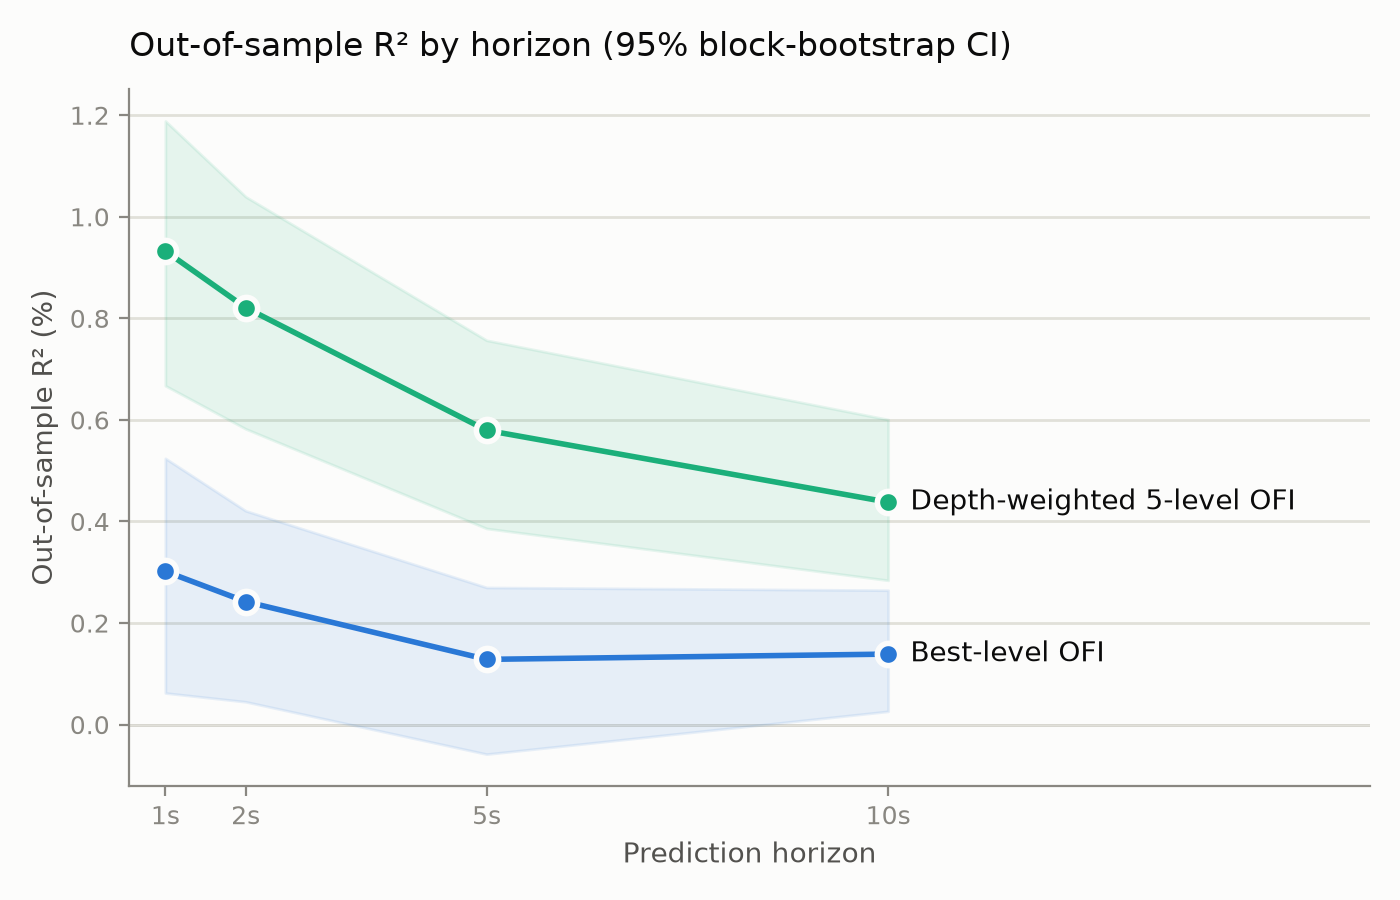
\includegraphics[width=0.85\textwidth]{figures/r2_vs_horizon.png}
\caption{Out-of-sample $R^2$ by horizon, 95\% block-bootstrap CI ($\sim$16-day sample, purge/embargo, gap-aware targets).}
\end{figure}

\subsection{A second data-quality finding, caught the same way as the first}

The first pass at this extension (before the fix described above) produced one walk-forward fold with an out-of-sample $R^2$ of \textbf{$-$3{,}671\%} (best-level OFI, 1s horizon) --- not a typo, three orders of magnitude beyond anything economically meaningful. Inspecting that fold's test period directly showed every single row (139{,}430 of them) had $n_{events} = 0$, \texttt{mid\_price\_filled} = True, and consequently \texttt{fwd\_ret\_1s} exactly $0.0$: the fold's entire test window fell inside the $\sim$3-day-21-hour collector outage from \S2.1, where \texttt{aggregate\_windows} had correctly flagged the forward-filled placeholder price but nothing downstream had excluded it. A near-zero benchmark SSE (predicting the training mean against an actual value of exactly zero, repeated) divided into an also-tiny-but-larger model SSE produced an enormous ratio --- small in absolute terms, which is why the \emph{pooled} headline numbers in \S4.3 barely moved (well within their own confidence intervals) once fixed, but arbitrarily large in relative terms, which is why the per-fold breakdown was unusable without the fix.

We flag this as a second instance of the same pattern as \S2.2: a silent, non-crashing data issue that produced no exception anywhere in the pipeline, caught only because we routinely decompose pooled statistics fold-by-fold rather than trusting an aggregate number on its own. The fix (\S3.2) NaNs any target touching a filled window before it ever reaches the walk-forward splitter; the affected fold now correctly contributes zero rows rather than a fabricated result.

\subsection{Fold-level diagnosis (post-fix)}

Repeating the fold-by-fold decomposition on the corrected \S4.3 sample (best-level and multi-level OFI, 1s horizon; fold 2 is the now-excluded outage fold):

\begin{table}[h]
\centering
\begin{tabular}{lrrrrr}
\toprule
Fold & Valid $n$ & Fitted $\beta$ (best) & OOS $R^2$ (best) & Fitted $\beta$ (multi) & OOS $R^2$ (multi) \\
\midrule
0 & 113{,}830 & 0.000038 & $-$0.29\% & 0.000027 & +0.17\% \\
1 & 33{,}672 & 0.000030 & $-$0.22\% & 0.000023 & $-$0.16\% \\
2 & 0 & --- & (skipped) & --- & (skipped) \\
3 & 36{,}822 & 0.000029 & +1.24\% & 0.000022 & +2.31\% \\
4 & 113{,}908 & 0.000030 & +0.85\% & 0.000023 & +1.66\% \\
\bottomrule
\end{tabular}
\caption{Fold-by-fold decomposition, post-fix, both feature variants, 1s horizon.}
\end{table}

As in \S4.2, the fitted coefficient never changes sign in either feature (0.000038$\to$0.000030 best-level; 0.000027$\to$0.000023 multi-level) --- small, stable, slowly drifting, not flip-flopping. Fold-level fit is still uneven (two negative, two positive, of noticeably different magnitude --- fold 3's smaller sample in particular swings hardest in both directions), but the positive folds now outweigh the negative ones enough that the pooled result in \S4.3 is positive with most CIs excluding zero, rather than the roughly even split that produced \S4.2's null result. This is consistent with a real effect that becomes detectable once enough folds are pooled, rather than with either ``no effect'' or ``unstable-sign effect.''

\section{Discussion}

The result changed direction twice across three extensions of the identical capture and pipeline: positive (\S4.1) $\to$ null/negative (\S4.2) $\to$ positive again, with two fixed data bugs and a stricter validation methodology (\S4.3--4.5). We think the most defensible reading is not ``the effect is real'' or ``the effect is fake,'' but that \textbf{a linear OFI effect at these horizons on this venue, if it exists, sits close enough to the detection threshold for a single-symbol, single-venue sample that whether a given $\sim$1--2 week window shows it depends heavily on which specific days that window contains.} The coefficient's sign and rough magnitude were stable across every fold in every phase of this study; what varied was whether out-of-sample fit happened to net positive or negative once pooled --- exactly what you'd expect from a small true effect competing with day-to-day noise, not from a spurious or regime-reversing relationship.

This instability is also the paper's central methodological point, and it held at two different scales. The \S4.1 result passed every check available at the time --- correct sign, monotonic decay, significant Newey-West $t$-stats, a bootstrap CI excluding zero, a passed placebo test --- and still reversed on more data. The \S4.3 result passed the same battery of checks, this time with purge/embargo added, and its fold-level decomposition (\S4.5) is markedly less clean than \S4.1's would suggest at a glance: two of four valid folds are still negative. Separately, the fold-level habit itself caught a second, unrelated data bug (\S4.4) that would otherwise have sat invisibly inside a ``validated'' pipeline. None of this would have surfaced from the pooled headline number alone at any stage.

\section{Limitations}

\begin{itemize}
\item \textbf{Single symbol, single venue.} BTC/USDT on Binance.US only. Binance.US has materially lower volume than Binance.com's international venue; results may not generalize to more liquid venues or other symbols.
\item \textbf{Sample length and composition.} $\sim$16 days is still short given the fold-to-fold variance in \S4.5, and roughly a quarter of the extended capture window was unusable (collector outage). We cannot yet rule out that the current positive result is itself sample-dependent in the same way \S4.1's was.
\item \textbf{Linear model only.} We tested plain OLS on the raw OFI value. A nonlinear specification, interaction terms, or additional order-book features (spread, depth imbalance, recent realized volatility) might extract signal a single linear term cannot.
\item \textbf{No transaction costs.} This is a pure statistical predictability study, not a trading strategy evaluation --- even where OOS $R^2$ is positive and significant, that would not by itself imply a profitable strategy net of fees, spread-crossing costs, and latency.
\item \textbf{Multi-level weighting is a design choice.} The $1/i$ depth-weighting scheme for the 5-level OFI variant is not from the original paper; other weightings (equal-weight, liquidity-weighted) were not tested and might behave differently.
\item \textbf{The collector is not fault-tolerant to being closed.} It is a foreground process; the 3-day-21-hour gap in \S2.1 was an operational failure (a closed terminal), not a WebSocket-level one, and would recur without a supervised/background deployment.
\end{itemize}

\section{Conclusion}

Across three successive extensions of the same BTC/USDT L2 capture from Binance.US ($\sim$7, $\sim$9, and $\sim$16 days), evaluated with an identical walk-forward pipeline that was tightened along the way (purge/embargo, gap-aware targets), the out-of-sample evidence for OFI predicting 1--10 second returns went positive, then null, then positive again --- each time significant on the same battery of checks, including a permutation placebo. Fold-level decomposition throughout is consistent with a small, direction-stable, hard-to-detect effect rather than either ``no relationship'' or a spurious one, and separately surfaced a second silent data-pipeline bug (unmasked targets across a multi-day collection outage) using the same diagnostic habit that flagged the first (\S2.2). We treat the current positive result as provisional, not confirmed --- precisely because an earlier positive result on this same growing capture already reversed once. The natural next step is the same one that has mattered at every stage so far: more data, and another deliberate attempt to break the result before trusting it.

\begin{thebibliography}{9}

\bibitem{cks2014}
Cont, R., Kukanov, A., \& Stoikov, S. (2014). The Price Impact of Order Book Events. \emph{Journal of Financial Econometrics}, 12(1), 47--88.

\bibitem{ct2008}
Campbell, J. Y., \& Thompson, S. B. (2008). Predicting Excess Stock Returns Out of Sample: Can Anything Beat the Historical Average? \emph{Review of Financial Studies}, 21(4), 1509--1531.

\bibitem{nw1987}
Newey, W. K., \& West, K. D. (1987). A Simple, Positive Semi-Definite, Heteroskedasticity and Autocorrelation Consistent Covariance Matrix. \emph{Econometrica}, 55(3), 703--708.

\bibitem{kunsch1989}
Kunsch, H. R. (1989). The Jackknife and the Bootstrap for General Stationary Observations. \emph{The Annals of Statistics}, 17(3), 1217--1241.

\bibitem{lopezdeprado2018}
L\'opez de Prado, M. (2018). \emph{Advances in Financial Machine Learning}. Wiley. (Purge/embargo, ch.\ 7.)

\end{thebibliography}

\section*{Reproducibility}

All code is in the accompanying repository. To reproduce the \S4.3--4.5 result from raw capture:

\begin{verbatim}
python -m src.orderbook --raw data/raw --out data/processed/book
python -m scripts.run_ofi_study --processed data/processed/book --out reports/results.csv
python -m scripts.make_figures --results reports/results.csv --out-dir paper/figures
\end{verbatim}

\texttt{pytest} runs the full test suite (order-book reconstruction, OFI formula, window/target alignment, gap masking, walk-forward chronology and purge/embargo, and evaluation-statistics tests against synthetic data with known-correct answers; 47 cases as of this draft).

\end{document}
